\documentclass{article}

\usepackage[utf8]{inputenc}
\usepackage{graphicx}
\usepackage{multirow}
 \usepackage{url}
% correct bad hyphenation here

\hyphenation{pre-sence vi-su-alized si-mu-la-tions mo-le-cu-lar se-ve-ral cha-rac-te-ris-tic CoNSEnsX}

\title{Önálló laboratórium:\\Áramlástani folyamatok modellezésének gyorsítása FPGA-n}
\author{\IEEEauthorblockN{Tóth András (UHTG2J)\\Konzulens: dr. Nagy Zoltán\\Pázmány Péter Katolikus Egyetem\\Információs Technologiai és Bionikai Kar\\Mérnökinformatikai képzés\\
\texttt{tothdonci0@gmail.com}}
}
\usepackage[arrowdel]{physics}


\begin{document}

\maketitle
\tableofcontents

\section{Áramlási model}
\subsection{Egyenletek}
 \cite{article} A Navier-Stokes egyenletek, folyadékok tulajdonságait leíró egyenetrendszer (tömeg, momentum, energia-megmaradás, kibővítve a disszipációs hatások, a viszkozitás, a diffúzió és a hőátadással). Ha nem vesszük figyelembe a nem ideális körülményeket és adiobatikus rendszert feltételezünk, az Euler-egyenleteket kapjuk. Ezek az egyenletek hiperbolikus parciális differenciál egyenletek.


\begin{equation} \label{eq1}
\begin{split}
\frac{\partial \rho}{\partial t}+\grad \cdot (\rho \mathbf{v}) = 0 \\
\frac{\partial(\rho \mathbf{v})}{\partial t}+\grad \cdot (\rho \mathbf{vv}+\widehat{I} p) = 0 \\
\frac{\partial E}{\partial t}+\grad \cdot ((E+p)\mathbf{v}) = 0
\end{split}
\end{equation}
\label{eq2}
ahol $t$ az idő, $\grad$ a nabla operátor, $\rho$ a sűrűség, $u$, $v$ rendre a $v$ sebesség vektor $x$ és $y$ komponensei, $p$ a gáz/folyadék nyomása, $\widehat{I}$ az egység mátrix és $E$ a teljes energia sűrűség, amit az alábbi egyenlet határoz meg:
\begin{equation}
    E = \frac{p}{\gamma-1}+\frac{1}{2}\rho \mathbf{v} \cdot \mathbf{v}
\end{equation}
A \ref{eq2} egyenletben $\gamma=1.4$. Későbbi felhasználásra bevezetjük a konzervatív állapot vektort $U =[\rho,\rho u,\rho v, E]$, a primitív változókat $P=[\rho,u,v,E]$ és a hang sebességét $c=\sqrt{\gamma p/ \rho}$

\ref{eq1}. egyenletrendszert $U$ és $F$ fluxus tenzort felhasználva össze vonhatjuk:
\begin{equation}
\label{eq3}
\mathbf{F}=\begin{pmatrix}
\rho \mathbf{v}\\ \rho \mathbf{v v} +I p 
\\ (E+p)v

\end{pmatrix}
\end{equation}
, mint
\begin{equation}
\label{eq4}
    \frac{\partial U}{\partial t}+\grad \cdot \mathbf{F}=0
\end{equation}
\subsection{A háló gemometriája}
$\Omega$ a modellezett tér. Esetünkben ez téglalap alakú. $\Omega$-t $M\times N$ nem átfedő, egyenlő méretű cellákra osztjuk.  A téglalapok oldalai $a$ és $b$ egység hosszúak. (i,j) az i-edik sorban és j-edik oszlopban szereplő cellát jelenti.

A háló felbontását x és y irányokban, figyelembe véve a terület méreteit $\Delta x=a/M$ és $\Delta y =b/N$ jelenti, így (i,j) cella paraméterei $V_{i,j}$.
\subsection{Diszkretizáció}
\ref{eq4}. egyenletet diszkretizálva 
\begin{equation}
    \label{eq5}
    \frac{\mathrm{d}U_{i,j}}{\mathrm{d}t}=-\frac{1}{V_{i,j}} \sum_{f}{}\mathbf{F}_{f}\cdot \mathbf{n}_{f}
\end{equation}
ahol a szummát a cella mind a 4 oldalára értendő (i,j), $\mathbf{F}_{f}$ a fluxus tenzor, melyet a cella $f$ oldalán kiértékelendő és $\mathbf{n}_{f}$ a kifelé mutató  normál vektor.

\begin{figure}[ht]
\begin{center}
\caption{\cite{article} Cellák és normálvektorok, melyek szükségesek a számításhoz}
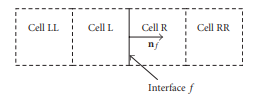
\includegraphics[scale=1]{image.png}
\label{fig:1}
\end{center}
\end{figure}

\cite{article} cikk végül az alábbi diszkrét egyenlet rendszerre jut, ahol F a numerikus fluxus és D a disszipáció:

\begin{equation}
    \begin{split}
        F^{\rho , n }_{i}=\frac{\rho u^{n}_{C}+\rho u^{n}_{i}}{2}, i=E,W \\
        F^{\rho u, n }_{i}=\frac{(\rho u^{2}+p)^n_{C}+(\rho u^{2}+p)^n_{i}}{2}, i=E,W \\
         F^{\rho u, n }_{i}=\frac{\rho u v^{n}_{C}+\rho u v^{n}_{i}}{2}, i=N,S\\
          F^{\rho v, n }_{i}=\frac{\rho u v^{n}_{C}+\rho u v^{n}_{i}}{2}, i=E,W \\
          F^{\rho v, n }_{i}=\frac{(\rho v^{2}+p)^n_{C}+(\rho v^{2}+p)^n_{i}}{2}, i=N,S \\
          F^{E, n }_{i}=\frac{(E+p) u^n_{C}+(E+p) u^n_{i}}{2}, i=E,W \\
          F^{E, n }_{i}=\frac{(E+p) v^n_{C}+(E+p) v^n_{i}}{2}, i=N,S \\
          D^{\rho , n }_{i}=(| \bar{u}|+\bar{c}) \frac{\rho^{n}_{i}-\rho^{n}_{C}}{2},i=E,N\\
          D^{\rho , n }_{i}=(| \bar{u}|+\bar{c}) \frac{\rho^{n}_{C}-\rho^{n}_{i}}{2},i=W,S\\
          D^{\rho u, n }_{i}=(| \bar{u}|+\bar{c}) \frac{\rho u^{n}_{i}-\rho u^{n}_{C}}{2},i=E,N\\
           D^{\rho u, n }_{i}=(| \bar{u}|+\bar{c}) \frac{\rho u^{n}_{C}-\rho u^{n}_{i}}{2},i=W,S\\
            D^{\rho v, n }_{i}=(| \bar{u}|+\bar{c} )\frac{\rho v^{n}_{i}-\rho v^{n}_{C}}{2},i=E,N\\
             D^{\rho v, n }_{i}=(| \bar{u}|+\bar{c} ) \frac{\rho v^{n}_{C}-\rho v^{n}_{i}}{2},i=W,S\\
              D^{\rho E, n }_{i}=(| \bar{u}|+\bar{c}) \frac{E^{n}_{i}-E^{n}_{C}}{2},i=E,N\\
               D^{E, n }_{i}=(| \bar{u}|+\bar{c}) \frac{E^{n}_{C}-E^{n}_{i}}{2},i=W,S\\
    \end{split}
\end{equation}
\subsection{Léptetési séma}
\begin{equation}
    \begin{split}
        \rho^{n+1}_{C}=\rho^{n}_{C}-\frac{\Delta t}{\Delta x}(F^{\rho n}_{E}-F^{\rho ,n}_{W}+D^{\rho ,n}_{E}-D^{\rho ,n}_{W})-\frac{\Delta t}{\Delta y}(F^{\rho ,n}_{N}-F^{\rho ,n}_{S}+D^{\rho ,n}_{N}-D^{\rho ,n}_{S}), \\
        
                \rho u^{n+1}_{C}=\rho u^{n}_{C}-\frac{\Delta t}{\Delta x}(F^{\rho u ,n}_{E}-F^{\rho u,n}_{W}+D^{\rho u,n}_{E}-D^{\rho u,n}_{W})-\frac{\Delta t}{\Delta y}(F^{\rho u,n}_{N}-F^{\rho u,n}_{S}+D^{\rho u,n}_{N}-D^{\rho u,n}_{S}), \\
                
                \rho v^{n+1}_{C}=\rho v^{n}_{C}-\frac{\Delta t}{\Delta x}(F^{\rho v ,n}_{E}-F^{\rho v,n}_{W}+D^{\rho v,n}_{E}-D^{\rho v,n}_{W})-\frac{\Delta t}{\Delta y}(F^{\rho v,n}_{N}-F^{\rho v,n}_{S}+D^{\rho v,n}_{N}-D^{\rho v,n}_{S}), \\
                
                E^{n+1}_{C}=E^{n}_{C}-\frac{\Delta t}{\Delta x}(F^{E ,n}_{E}-F^{E,n}_{W}+D^{E,n}_{E}-D^{E,n}_{W})-\frac{\Delta t}{\Delta y}(F^{E,n}_{N}-F^{E,n}_{S}+D^{\rho v,n}_{N}-D^{\rho v,n}_{S}), \\
    \end{split}
\end{equation}

\section{Optimalizációs tehnikák}
\cite{hls} \cite{optim} Vitis HLS különböző direktívákat támogat a különböző metrikákhoz, ami a kívánt teljesítményt segít elérni.
\begin{itemize}
    \item Pipelining: a következő függvény indulhat hogy az előző még nem ért véget
    \item Cél késleltetés mgatározása
    \item Erő forrás limit mghatározása
    \item I/O protokoll meghatározása, hogy a függvény paraméterek, más eszközök outputjára lehessen kötni bármilyen protokollal. 
\end{itemize}
Ezeket  tehnikákat aszerint csoportosíthatjuk, hogy mely teljesítmény metrikát célozza.

Néhány optimalizációs direktíva a teljsség igénye nélkül:
\begin{itemize}
    \item \textbf{AGGREGATE}: egy struct minden elemét eggyetlen vekorba tömöríti, hogy lhessen egyszerre írni és olvasni
    \item \textbf{PIPELINE}: for-cikluson bellül párhuzamosít feladatokat
    \item \textbf{INTERFACE}: Meghatározza az RTL portok hogyan jönnek létre a fügvény leírásból.
    \item \textbf{LATENCY}: Beállíthatunk minimum és maximum korlátot a késleltetésnek.
    \item \textbf{STREAM}: Meghatározza hogy egy adott array FIFO vagy RAM memória csatorna az adatfolyam optimalizáció során. 
    \item \textbf{TOP}: Az a függvény amit szintetizálunk az alfüggvényeivel együtt. Több top-level függvény megadása tulajdonképpen lehetővé tesz több solution-t egy projekten bellül.
    \item \textbf{UNROLL}: Egy for-ciklus kigöngyölése során a ciklus testét többször létrehozza, majd azt párhuzamosítani tudja függetlenül egymástól.
\end{itemize}

\subsection{Pipeline}
\begin{figure}[ht]
\begin{center}
\caption{\cite{hls} \cite{optim} Függvény Pipeline}
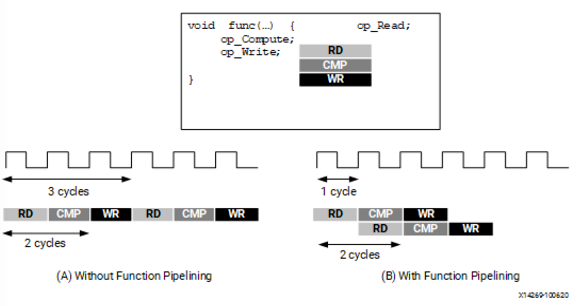
\includegraphics[scale=1]{pipeline.PNG}
\label{fig:2}
\end{center}
\end{figure}
\begin{itemize}
\item \textbf{Függvény pipeline példa}
\cite{hls} \cite{optim} \ref{fig:2}. képen látható a példa.
Példánkban pipeline nélkül a függvény 3 órajel ciklus alatt olvas be egy input-ot és 2 órajel ciklus alatt ad output-ot. A függvénynek 3 az inicialaizációs intervalluma és 3 a késleltetése.

Pipeline-al új input-ot olvas minden ciklusban és a késleltetésben még sincs változás. Ciklus pipeline-olás miatt a ciklus magjában lévő műveletek párhuzamosan futnak.

\ref{fig:2}. képen látható, hogy eredetileg 3 órajel ciklus volt a késleltetés minden beolvasás között és 8 órajel ciklus kell neki mire az utolsó kiírás lefut.

A pipeline-olt változatában a ciklusnak, minden ciklusban egy új input kerül beolvasásra minden órajel ciklus során és a kimenetre 4 órajel ciklus után ír. Ezzel a módszerrel lényegesen csökkentve a késleltetését a függvénynek, pedig lényegében ugyan azt a hardware-t használják.

\ref{fig:3}. kép a ciklusok pipline-olását mutatja be.

\item \textbf{Ciklus és függvény pipeline különbsége:}
\begin{figure}[ht]
\begin{center}
\caption{\cite{hls} \cite{optim} Ciklus pipeline}
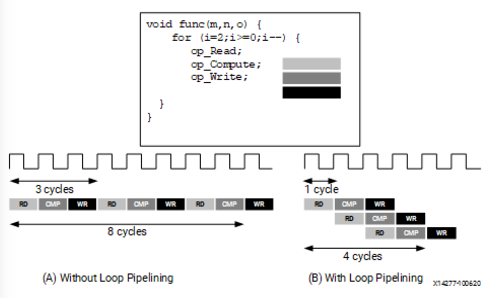
\includegraphics[scale=1]{cilus_pipeline.PNG}
\label{fig:3}
\end{center}
\end{figure}
A direktívát a konkrét régióra kell megadni, ahol a függvény vagy ciklus teste megvalósításra kerül. Mert nem érinti az egész hierarchiát alatta, csak és kizárólag a régióra vonatkozik. Ugyanakkor az alatta fekvő teljes hierarhiában az összes ciklust automatikusan unroll-olja (Unroll-ról lásd később). A hierarchiában alatta minden al-függvényt külön-külön kell pipeline-olni. Ha az alfüggvény pipeline-olva van, pipeline-olt függvény fölötte kihasználhatja ezt. Ugyanakkor ha bármely al-fügvény nincs pipline-olva, az egy korlátozó tényező lehet a pipeline teljesítményére nézve.

Van különbség a pipeline-olt függvények és ciklusok viselkedésében.

Pipeline-olt függvény minden ciklusban kaphat új bemeneti adatot. Ha nem kap "exit"-et akkor nem áll meg.
Pielone-olt ciklus addig fut amíg az összes iteráció le nem futott.
Ezt a különbséget a \ref{fig:5}. kép összegzi.
\begin{figure}[ht]
\begin{center}
\caption{\cite{hls} \cite{optim} Ciklus és Függvény pipeline különbsége}
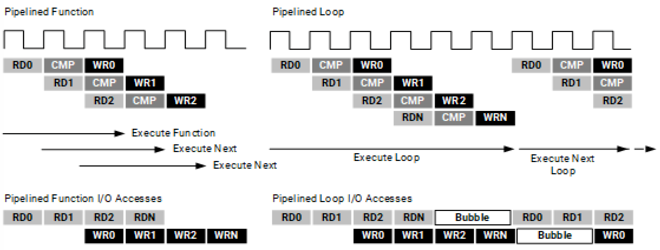
\includegraphics[scale=0.7]{difference.PNG}
\label{fig:5}
\end{center}
\end{figure}
\item \textbf{Függvény és ciklus pipeline interakciója:}
A viselkedésbeli különbségek meghatározzák, a pipeline bemenetének és kimenetének feldolgozását. Ahogy a \ref{fig:5}. kép mutatja, egy pipeline-olt függvény folyamatosan új input-okat olvas és output-okat ír.

Viszont a ciklusok iterációi nem függetlenek egymástól. Ezért a ciklusnak a következő iteráció előtt minden műveletet el kell végeznie. Egy pipeline-olt ciklus amolyan "buborékot" képez az adatfolyamban, egy pontot ahol nem olvas új input-okat, míg a  ciklus elvégzi a műveleteket és egy pontot ahol nem ír ki output-okat, amíg új iterációkat indít a ciklus.
\end{itemize}
\subsection{Unroll}

\begin{figure}[ht]
\begin{center}
\caption{\cite{hls} \cite{optim} Unroll}
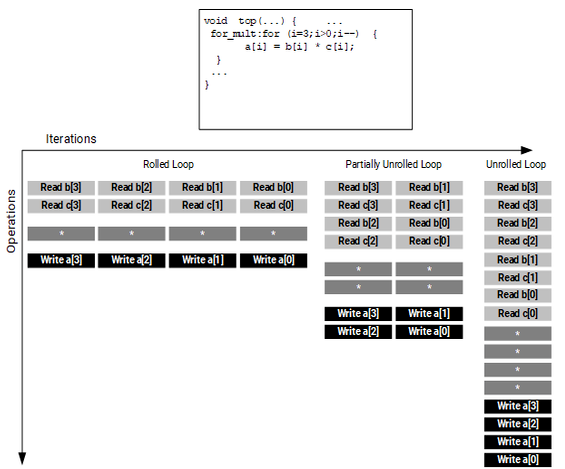
\includegraphics[scale=0.7]{Unroll.PNG}
\label{fig:4}
\end{center}
\end{figure}
"Kigöngyölés"-ként fogok a műveletre referálni ebben a fejezetben a magyarázat kedvéért.

Vitis HLS alapból a ciklusokat begöngyölve tartja. Ezek a begönygyölt ciklusok egy hardware-es erőforrást használnak, melyet minden iteráció használ. Bár ez erőforrások szempontjából nagyon hatékony, teljesítmány szempontjából sajnos nem.

"Unroll" pragma vagy direktíva használatával egy for-ciklus teljesen, vagy részlegesen kigöngyölhető.

\ref{fig:4}. ábra mutatja a kigöngyölés előnyeit és következményeit. 

\section{Hardver: Zynq-7000}
\cite{Hardware} \cite{Hardware2}
Xilinx arhitektúrán alapszik. Egy eszközön integrálja ARM Cortex - A9 MPCore  alapú PS-t (processing system) és a Xilinx PL-t (progammable logic).
MPCore CPU-k a szive(i) a PS-nek ami tartalmaz továbbá belső memóriát és külső memória interface-eket és I/O perifériák gazdag választékát.

A processzorok a PS-ben mindig először boot-olnak ami szoftver centrikus megközelítést tesz lehetővé a PL indításához és konfigurálásához. A PL-t lehet indítási folyamat részeként is, vagy akár később is konfigurálni. 

A rendszer előnye az FPGA flexibilitása és skálázhatósága. Kivállóan alkalmas költség hatékony és nagy teljesítményű aplikációk tervezésére egyaránt. Xilinx és társai széleskörűen támogatják fejlesztői környezetekkel, példa kódokkal.

\section{Teljesítmény metrikák}
\cite{hls}
\begin{itemize}
    \item Felület
    
    \begin{itemize}
        \item logikai erőforrások (LUT, register)
        \item Block RAM
        \item DSP slice
    \end{itemize}
    
    \item Késleltetés: órajelek száma ami alatt a fügvény számol
    \item Újraindítási sebesség: órajelek száma ami alatt a függvény új inputot kap
\end{itemize}

\section{Software}
3 fő komponens:

\subsection{Kommunikáció}
c++ nyelvben van leírva, mert ARM processzoron fut, ami tud TCP/IP protokollal kommunikálni, ezt FPGA-n külön projekt lenne felépíteni és nem is lenne hatékony. Csatlakozni pythonban írt klienssel lehet, mert azzal könnyen lehet plotolni az eredményeket.

\begin{itemize}
\item Futtat egy ciklust ami poll-olja a bejövő utasításokat.
\item Számon tart egy státuszt amit kliens lekérhet.
\item Kliens leállíthatja a programot.
\item Kliens inputot küldhet. Ehhez előbb a formátumot küldi el, majd a paramétereket.
\item Kliensnek elküldheti a számított eredményeket.
\end{itemize}

\subsection{Kernel}
\cite{projekt} Diszkretizált áramlási modellt kódolja le. Léptetési séma alapján mozgat, iterációnként "egyet". Jelenleg majdnem egy az egyben dr. Nagy Zoltán tanár úr cfd\_struct projektje. Ez 2 dimenziós, tervek szerint 3 dimenzióssá bővítem. 

\cite{intro} Vitis HLS támogatja a C/C++ nyelvet mely kiváltja így a VHDL-t. A C kódot RTL leírássá fordítja. Ez megkötéseket jelent. Mert minden kód részlet egyértelmű áramkört kell eredményezzen pont ahogy a VHDL nyelv tenné. Erre egy példa C oldalról, hogy a Vitis HLS C/C++ implementációban a top-level függvény szigoruan nem tartalmazhat Template-et (generikus struktúrát), ennek ellenére szerencsére a kód egyéb részei tartalmazhatnak. 

\subsection{Vezérlő kód}
 Az FPGA-ra integrált ARM processzor tud az FPGA-val kommunikálni OpenCL függvény hívásokkal. Azon több kernelt is képes lenne futtatni és egy array-ben kezeli őket (esetünkben csak egy kernel van a cfd\_struct). A TCP/IP kommunikációt végző struktúra és az FPGA közötti kommunikációt végzi. Betölti a megfelelő bufferekből a kapott paramétereket és OpenCL függvényhívással leküldi a kernelnek. És az outout-ot vissza propagálja a kommunikátornak. 

\begin{thebibliography}{9}
\bibitem{balzek}
Jiri Blazek: Computational Fluid Dynamics Principles

\bibitem{article}
Kocsárdi Sándor, Nagy Zoltán, Csík Árpád és Szolgay Péter: Simulation of Two-Dimensional Supersonic Flows on Emulated-Digital CNN-UM EURASIP J. Adv. Signal Process. 2009, 923404 (2009). \\https://doi.org/10.1155/2009/923404

\bibitem{hls}
High-level synthesis methods on FPGA-s (MSC tantárgy)
\bibitem{fpga}
FPGA based algorith design (BSC tantárgy)
\bibitem{xilinx}
Vitis Unified Software Platform Documentation (UG1416) \\https://docs.xilinx.com/v/u/en-US/ug1416-vitis-documentation
\bibitem{optim}
Vitis High-Level Synthesis User Guide (UG1399) - Optimization Techniques in Vitis HLS \\https://docs.xilinx.com/r/en-US/ug1399-vitis-hls/Optimization-Techniques-in-Vitis-HLS
\bibitem{examples}
Xilinx/Vitis-HLS-Introductory-Examples \\https://github.com/Xilinx/Vitis-HLS-Introductory-Examples/tree/master/Pipelining
\bibitem{projekt}
cfd\_struct repository \\https://dev.itk.ppke.hu/cfd/cfd\_struct\_2d/-/tree/master/cfd\_struct\_2d\_hls
\bibitem{intro}
Vitis High-Level Synthesis User Guide (UG1399) - Itroduction 
\\ https://docs.xilinx.com/r/en-US/ug1399-vitis-hls/Introduction
\bibitem{Hardware}
Zynq-7000 SoC Data Sheet: Overview \\https://docs.xilinx.com/v/u/en-US/ds190-Zynq-7000-Overview
\bibitem{Hardware2}
Zynq-7000 SoC Technical Reference Manual (UG585) \\https://docs.xilinx.com/v/u/en-US/ug585-Zynq-7000-TRM
\end{thebibliography}
\end{document}